\chapter{B-Trees}
I B-tree sono alberi bilanciati di ricerca particolarmente utili poiché  progettati per essere memorizzati sui dischi. Poiché questi dischi sono molto più lenti della memoria ad accesso casuale (RAM), le prestazioni dei B-alberi vengono misurate non soltanto in base al tempo computazionale richiesto per eseguire le operazioni sugli insiemi dinamici, ma anche in base al \textbf{numero di accessi al disco}.
Poiché il numero di accessi al disco aumenta con l'altezza dell'albero, ciò che si fa' è avere un'altezza quanto più bassa possibile grazie ad un elevato numero di chiavi per nodo. Per cui, se gli alberi rosso neri hanno al più $O(log_2n)$ altezza, i b-tree avranno $O(log_tn)$ altezza. 
\begin{figure}[H]
    \centering
    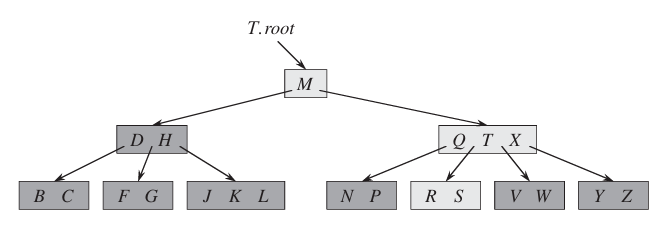
\includegraphics[width=0.5\linewidth]{Images/capitolo_3/b_tree_esempio.png}
    \label{fig:b_tree_esempio}
\end{figure}
\section{Ottimizzazione su Hard Disk}
Come accennato, questa struttura dati è parecchio utili perché ottimizza gli accessi all'hard disk. Un'hard disk è composto da più piatti uno sopra l'altro che girano attorno ad una asse comune e, questi, vengono letti mediante un'apposita testina che viene mossa da dei bracci meccanici. Per ammortizzare gli elevati tempi di posizionamento delle testine nelle tracce, le informazioni sono organizzate sui cilindri mediante blocchi della stessa dimensioni dette \textbf{pagine}. Risulterà quindi conveniente organizzare le strutture dati in maniera tale che queste sfruttino la suddivisione in pagine così ché gli accessi in lettura e scrittura avvengano solo su pagine intere. In tal senso, imposteremo i b-tree in maniera tale che un nodo abbia esattamente la dimensione di una pagina, così facendo, andremo a leggere al massimo $log_tn$ nodi che corrispondono all'altezza dell'albero.

\begin{figure}[H]
    \centering
    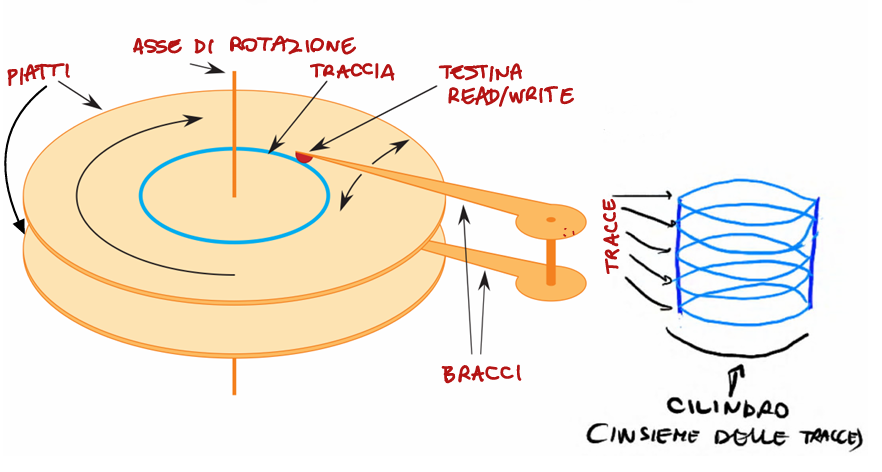
\includegraphics[width=0.5\linewidth]{Images/capitolo_3/hard_disk.png}
    \label{fig:hard_disk}
\end{figure}

\section{Definizione e altezza di un B-tree}
Un B-Tree T è un albero con radice in $root[T]$ che gode delle seguenti proprietà:
\begin{enumerate}
    \item Ciascun nodo $x$ ha i seguenti campi:
    \begin{itemize}
        \item n[x] numero delle chiavi in x ordinate in \textbf{ordine crescente} cioè $key_1[x]\leq key_2[x]\leq....\leq key_{n[x]}[x]$.
        \item leaf[x] campo booleano tale che è vero se x è una foglia e falso se è un nodo intero.
    \end{itemize}
    \item Ciascun nodo interno x contiene $n[x]+1$ puntatori ai figli indicati come $c_1[x], c_2[x],...,c_{n[x]+1}[x]$.
    \item Le chiavi $x.key_i$ separano gli intervalli delle chiavi memorizzate in ciascun sotto albero: Se $k_i$ denota una chiave nel sotto albero di radice $c_i[x]$ per $i=1,...,n[x]+1$, vale che $k_i\leq key_1[x]\leq k_2 \leq key_2[x] \le...\leq key_{n[x]}[x]\leq k_{n[x]+1}$. Proprio perché vale questa proprietà i b-tree sono alberi di ricerca. 
    \item Tutte le foglie hanno la stessa profondità che è l'altezza dell'albero.
    \item Ci sono limiti superiori e inferiori al numero di chiavi che si possono avere in un nodo. Questi possono essere espressi in base ad un intero $t\geq 2$ che è chiamato \textbf{grado minimo}.
    \begin{itemize}
        \item Ogni nodo, deve avere almeno $t-1$ chiavi. Ogni nodo interno, tranne la radice, quindi ha almeno t figli.
        \item Ogni nodo può contenere al massimo $2t-1$ chiavi. Quindi, un nodo interno
        può avere al massimo $2t$ figli. Diciamo che un nodo è pieno se contiene
        esattamente $2t-1$ chiavi.
    \end{itemize}
\end{enumerate}

\textbf{Teorema Altezza di un B-Albero}\\
Se $n\geq 1$, allora per qualsiasi B-Albero T di n chivi con altezza h e grado minimo $t\geq 2$, si ha che:
\[log_{2t}\frac{n+1}{2t}\leq h\leq\log_t\frac{n+1}{2}\]
Dimostriamolo:\\
Siano $n_h$ il minimo numero di chiavi e sia $N_h$ il massimo numero di chiavi. 
\begin{figure}[H]
    \centering
    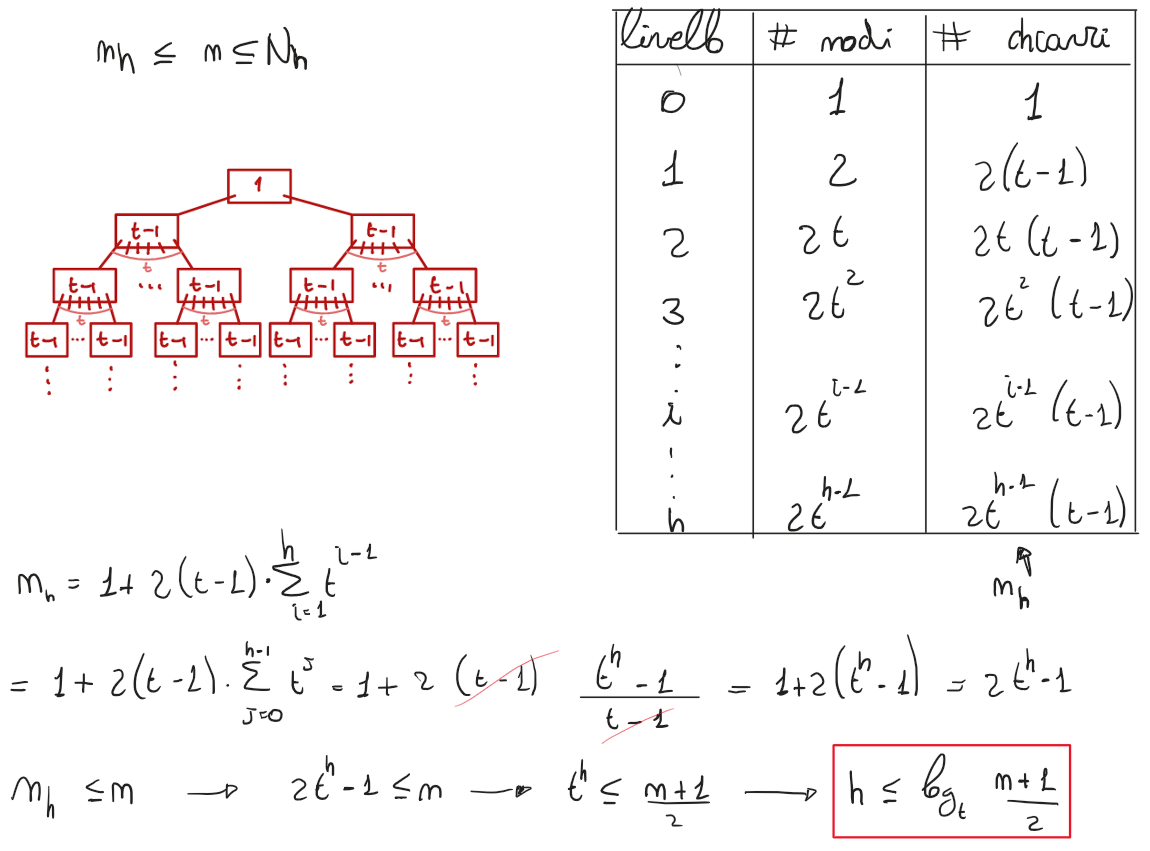
\includegraphics[width=1\linewidth]{Images/capitolo_3/dimostrazione_altezza_prima.png}
    \label{fig:altezza_prima}
\end{figure}
\begin{figure}[H]
    \centering
    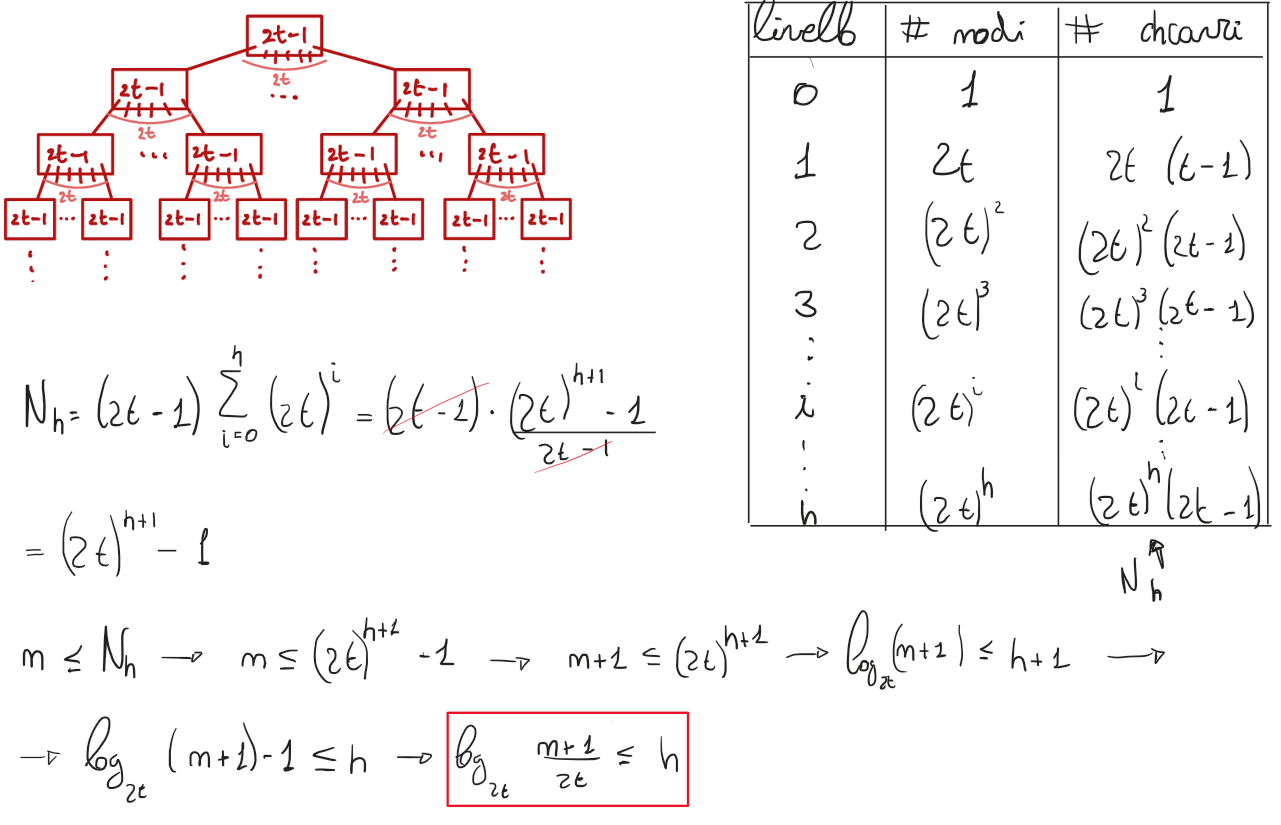
\includegraphics[width=1\linewidth]{Images/capitolo_3/dimostrazione_altezza_seconda.png}
    \label{fig:altezza_seconda}
\end{figure}
Da questi calcoli segue che $log_{2t}\frac{n+1}{2t}\leq h\leq\log_t\frac{n+1}{2}$ per cui si dimostra che $h=\Theta(log (n))$.

\section{Operazioni di base sui B-Tree}
Per quanto riguarda le operazioni sui B-Tree, descriveremo:
\begin{itemize}
    \item B-Tree-Search
    \item B-Tree-Create
    \item B-Tree-Insert
    \item B-Tree-Delete
\end{itemize}

Supporremo che la radice sia sempre in memoria e che per tutti i nodi passati come parametro deve essere chiamata la procedura read.\\
\section{B-Tree-Search(x,k)}
In questa procedura quello che sarà fatto sarà analizzare gli intervalli in un nodo e, nel caso il numero cercato fosse in quell'intervallo, si scende ancora con il nodo fino a quando non si trova ciò che si cerca.


\begin{algorithm}[H]
\caption{B-TREE-SEARCH($x$, $k$)}
\begin{algorithmic}[1]
    \State $i \gets 1$
    \While{$i \leq n[x]$ \textbf{and} $k > key_i[x]$} \Comment{Fino a quando la chiave corrente è minore}
        \State $i \gets i + 1$
    \EndWhile
    
    \If{$i \leq n[x]$ \textbf{and} $k = key_i[x]$} \Comment{Se non abbiamo analizzato tutte le chiavi e abbiamo trovato k}
        \State \Return $(x, i)$ \Comment{Allora abbiamo trovato la chiave cercata}
    \EndIf
    
    \If{$leaf[x]$} \Comment{Altrimenti, se il nodo è una foglia...}
        \State \Return \textbf{NIL} \Comment{...la chiave non è presente}
    \Else
        \State \textsc{Disk-Read}$(c_i[x])$ \Comment{Altrimenti, leggiamo da disco il figlio}
        \State \Return \textsc{B-TREE-SEARCH}$(c_i[x], k)$ \Comment{E cerchiamo ricorsivamente}
    \EndIf
\end{algorithmic}
\end{algorithm}

La complessità sarà $O(h)=O(log_tn)$ per quanto riguarda gli accessi al disco e $O(th)=O(tlog_tn)$ per quanto riguarda il tempo di cpu. \\
\section{B-Tree-Create}
Questa operazione consiste nella creazione di un albero vuoto per cui, semplicemente, andremo creare la radice.
\begin{algorithm}[H]
\caption{B-TREE-INITIALIZE()}
\begin{algorithmic}[1]
    \State $x \gets \text{Allocate-Node}()$ \Comment{Allocazione di un nuovo nodo}
    \State $leaf[x] \gets \text{true}$ \Comment{Il nodo appena creato è una foglia}
    \State $n[x] \gets 0$ \Comment{Numero di chiavi nel nodo inizialmente 0}
    \State \text{Disk-Write}($x$) \Comment{Scriviamo il nodo su disco}
    \State $root[T] \gets x$ \Comment{Impostiamo la radice dell'albero}
\end{algorithmic}
\end{algorithm}
\section{Inserimento in un B-Tree}
Si chiama innanzitutto la B-Tree-Search per localizzare la foglia dove fare l'inserimento e, se questa non è piena, allora si inserisce k nella posizione opportuna. Altrimenti, si divide la foglia in due, il mediano va' nel nodo sopra e la chiave si inserisce dov'è di giusto.
\begin{figure}[H]
    \centering
    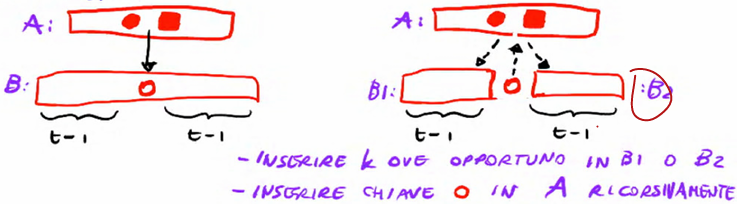
\includegraphics[width=0.8\linewidth]{Images/capitolo_3/inserimento_con_split.png}
    \label{fig:inserimento_con_split}
\end{figure}
Inoltre, per far sì che il tutto non risalga alla radice, si faranno le suddivisione mentre si scende per localizzare la foglia in cui inserire la chiave e si utilizzerà un'ulteriore procedura chiamata B-Tree-Split-Child(x,i) con x nodo non pieno e i nodo figlio di x.
\begin{algorithm}[H]
\caption{B-TREE-SPLIT-CHILD($x$, $i$)}
\begin{algorithmic}[1]
    \State $z \gets \textsc{Allocate-Node}()$ \Comment{Si crea un nuovo nodo}
    \State $y \gets x.c_i$ \Comment{Si identifica il nodo da dividere}
    \State $z.leaf \gets y.leaf$ \Comment{Il nuovo nodo prende lo stesso status di foglia di y}
    \State $z.n \gets t - 1$ \Comment{Il nuovo nodo avrà t-1 chiavi perché dividiamo un nodo pieno che ha al più 2t-1}
    \For{$j \gets 1$ \textbf{to} $t - 1$} \Comment{Le chiavi di y vengono divise dove c'è il mediano} 
        \State $z.key_j \gets y.key_{j+t}$
    \EndFor
    \If{\textbf{not} $y.leaf$} \Comment{Anche i puntatori ai sotto alberi si trasferiscono}
        \For{$j \gets 1$ \textbf{to} $t$}
            \State $z.c_j \gets y.c_{j+t}$
        \EndFor
    \EndIf
    \State $y.n \gets t - 1$ \Comment{Viene aggiornata anche la dimensione di y}
    \For{$j \gets x.n + 1$ \textbf{downto} $i + 1$}
        \State $x.c_{j+1} \gets x.c_j$
    \EndFor
    \State $x.c_{i+1} \gets z$ \Comment{Il nodo genitore viene aggiornato per accogliere z}
    \For{$j \gets x.n$ \textbf{downto} $i$} \Comment{Si shiftano per accogliere il mediano}
        \State $x.key_{j+1} \gets x.key_j$
    \EndFor
    \State $x.key_i \gets y.key_t$ \Comment{Si sposta il mediano}
    \State $x.n \gets x.n + 1$
    \State \textsc{Disk-Write}$(y)$ \Comment{Si salva il tutto}
    \State \textsc{Disk-Write}$(z)$
    \State \textsc{Disk-Write}$(x)$
\end{algorithmic}
\end{algorithm}

Questa procedura ha costo $O(1)$ per quanto riguarda gli accessi al disco e $\Theta(t)$ per quanto riguarda il tempo di CPU.

Analizzata questa procedura passiamo all'inserimento:
\begin{algorithm}[H]
\caption{B-TREE-INSERT($T$, $k$)}
\begin{algorithmic}[1]
    \State $r \gets T.root$
    \If{$r.n == 2t - 1$}
        \State $s \gets \textsc{Allocate-Node}()$ \Comment{Se la radice è piena, creiamo un nuovo nodo}
        \State $T.root \gets s$ \Comment{Che diventerà la nuova radice}
        \State $s.leaf \gets \textbf{false}$ 
        \State $s.n \gets 0$
        \State $s.c_1 \gets r$ \Comment{La vecchia radice diventa il nuovo figlio}
        \State \textsc{B-Tree-Split-Child}($s, 1$) \Comment{E il nuovo figlio viene diviso in due}
        \State \textsc{B-Tree-Insert-Nonfull}($s, k$) \Comment{Procedura a seguito}
    \Else
        \State \textsc{B-Tree-Insert-Nonfull}($r, k$) \Comment{Se il nodo non è pieno facciamo l'inserimento}
    \EndIf
\end{algorithmic}
\end{algorithm}

Come possiamo notare, vi è un'altra procedura che è B-Tree-Insert-Nonfull che effettua l'inserimento effettivo sul nodo non vuoto. In pratica questa procedura fa' si che si scenda sempre su un nodo non pieno, così facendo non abbiamo problemi nell'inserimento.
\begin{algorithm}[H]
\caption{B-TREE-INSERT-NONFULL($x$, $k$)}
\begin{algorithmic}[1]
    \State $i \gets x.n$
    \If{$x.leaf$} \Comment{Se è una foglia si inserisce subito}
        \While{$i \geq 1$ \textbf{and} $k < x.key_i$}
            \State $x.key_{i+1} \gets x.key_i$ \Comment{Le chiavi vengono shiftate per l'inserimento}
            \State $i \gets i - 1$
        \EndWhile
        \State $x.key_{i+1} \gets k$ \Comment{Si fa l'inserimento}
        \State $x.n \gets x.n + 1$
        \State \textsc{Disk-Write}($x$)
    \Else
        \While{$i \geq 1$ \textbf{and} $k < x.key_i$} \Comment{Viene determinato il figlio a cui scendere}
            \State $i \gets i - 1$
        \EndWhile
        \State $i \gets i + 1$
        \State \textsc{Disk-Read}($x.c_i$)
        \If{$x.c_i.n == 2t - 1$} \Comment{Se è pieno si effettua una split}
            \State \textsc{B-Tree-Split-Child}($x, i$)
            \If{$k > x.key_i$}
                \State $i \gets i + 1$
            \EndIf
        \EndIf
        \State \textsc{B-Tree-Insert-Nonfull}($x.c_i, k$) \Comment{Si rieffettua la chiamata per fare l'inserimento in un nodo non pieno}
    \EndIf
\end{algorithmic}
\end{algorithm}
Per quanto riguarda la complessità, avremo che la NonFull sarà $\Theta(h)$ per gli accessi al disco e $\Theta(th)$ per il tempo di CPU, per l'inserimento invece, avremo le stesse complessità. 

\section{Cancellazione da un B-Tree}
Per effettuare la cancellazione da un B-Tree innanzitutto utilizzeremo, anche qui, la procedura B-Tree-Search che ci indicherà il nodo dove si trova la chiave k da eliminare. Se tale nodo è una foglia con almeno t chiavi, allora si cancella la chiave, altrimenti, il nodo sarà definito \textbf{magro}, per cui avrà al massimo t-1 chiavi al suo interno e si dovrà procedere diversamente. Si andrà a guardare da una foglia sorella o dal nodo padre per verificare la possibilità di prestito di una chiave o di, eventualmente unione con un nodo sorella. 
\begin{figure}[H]
    \centering
    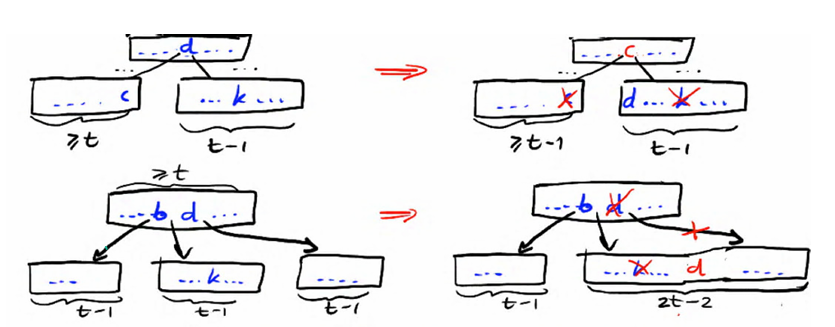
\includegraphics[width=0.8\linewidth]{Images/capitolo_3/cancellazione_b_tree.png}
    \label{fig:cancellazione_b_tree}
\end{figure}

Se il nodo contenente la chiave k è, invece, un nodo interno si sostituisce k con la chiave immediatamente più piccola e si cancelli il predecessore di k che risiederà su una foglia . Per evitare, anche in questo caso, di propagare il tutto fino alla radice, si farà in modo che i nodi del cammino dalla radice a k non siano magri. Pertanto:
\begin{enumerate}
    \item Se k è nel nodo x ed x è una foglia si cancella semplicemente k da x.
    \item Se k è nel nodo x ed x è interno:
    \begin{itemize}
        \item Se il figlio y di x che precede k ha almeno t chiavi, si determini il predecessore k' di k nel sotto albero radicato in y e lo si sostituisca a k. 
        \item Situazione simmetrica a quella di prima per il figlio z di x che segue k. In questo caso si prenderà il successore.
        \item Se sia y che z hanno t-1 chiavi, si uniscano k e il nodo z a y, si cancelli k da x, si deallochi z e si cancelli ricorsivamente da k e da y. 
    \end{itemize}
    \item Se la chiave non è presente sul nodo interno x, si determini la radice su cui continuare la ricerca:
    \begin{itemize}
        \item Se $c_i[x]$ è magro, si eseguano i passi 3 e si proceda ricorsivamente a eliminare k.
        \item Se $c_i[x]$ ha un fratello immediato non magro si proceda così:
        \begin{figure}[H]
            \centering
            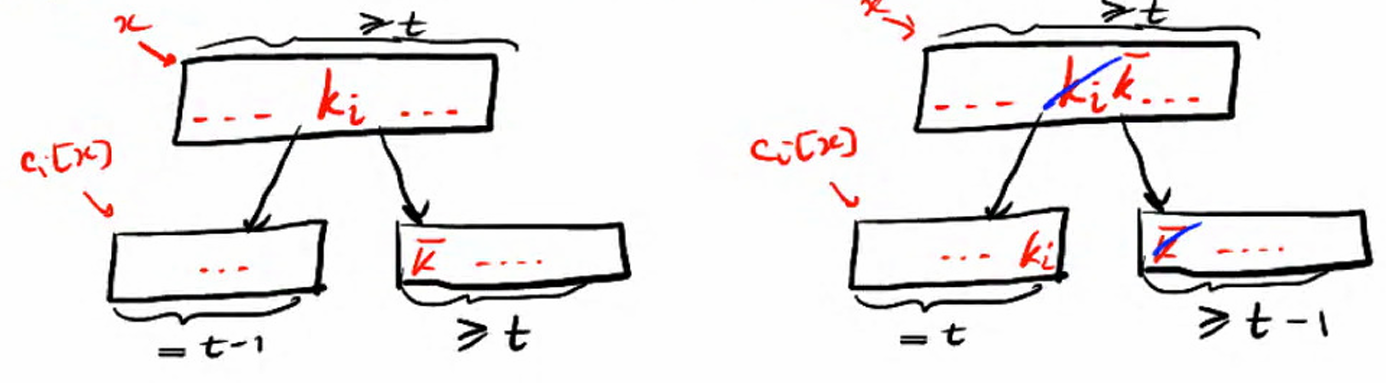
\includegraphics[width=0.8\linewidth]{Images/capitolo_3/cancellazione_cix_fratello_non_magro.png}
            \label{fig:fratello_non_magro}
        \end{figure}
        \item Se sono entrambi magri si proceda invece:
        \begin{figure}[H]
            \centering
            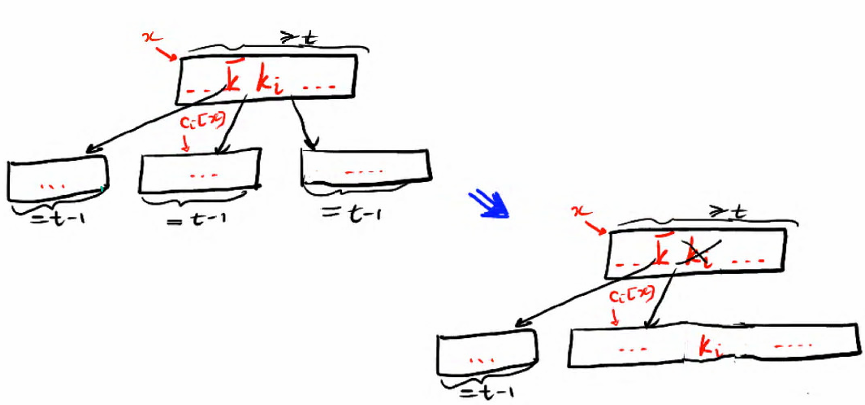
\includegraphics[width=0.8\linewidth]{Images/capitolo_3/fratelli_magri.png}
            \label{fig:fratelli_magri}
        \end{figure}
        \item Se $c_i[x]$ non è magro, si proceda ricorsivamente a cancellare la chiave k a partire dal nodo $c_i[x]$.
    \end{itemize}
\end{enumerate}


